\documentclass[conference,a4paper]{IEEEtran}
\usepackage[utf8]{inputenc}
\usepackage[T1]{fontenc}
\usepackage[spanish,es-noshorthands,es-tabla]{babel}
\usepackage{booktabs,graphicx,url}
\usepackage[hidelinks]{hyperref}
% Generado por bench/plot.py a partir de bench/results/. No editar a mano.
\newcommand{\NumEvents}{218\,841}
\newcommand{\NumReps}{3}
\newcommand{\NumRate}{2\,000}
\newcommand{\NumLatSeconds}{30}
\newcommand{\NumWarmup}{5}
\newcommand{\NumBatchEvery}{15}
\newcommand{\NumTpKappa}{32\,793}
\newcommand{\NumTpLambda}{22\,963}
\newcommand{\NumTpRatio}{1.4}
\newcommand{\NumRpKappa}{6.5}
\newcommand{\NumRpLambda}{0.61}
\newcommand{\NumBatchSeconds}{0.08}
\newcommand{\NumPfiftyKappa}{310}
\newcommand{\NumPfiftyLambda}{331}
\newcommand{\NumPninetynineKappa}{577}
\newcommand{\NumPninetynineLambda}{622}
\newcommand{\NumLocKappa}{119}
\newcommand{\NumLocLambda}{173}
\newcommand{\NumLocShared}{277}
\newcommand{\NumDbCpuKappa}{32}
\newcommand{\NumDbCpuLambda}{66}
\newcommand{\NumApiSeconds}{30}
\newcommand{\NumApiWarmup}{10}
\newcommand{\NumApiConc}{10 y 50}
\newcommand{\NumApiCmax}{50}
\newcommand{\NumApiReps}{3}
\newcommand{\NumRatioHourly}{7.8}
\newcommand{\NumRatioTop}{1.4}
\newcommand{\NumRatioPost}{3.4}
\newcommand{\NumTopKappaOverLambda}{3.3}
\newcommand{\NumMaxErr}{0.00}
\newcommand{\NumPostEvents}{10}
\newcommand{\EnvCpu}{AMD Ryzen 7 5700U with Radeon Graphics}
\newcommand{\EnvRam}{15}
\newcommand{\EnvDocker}{27.3.1}
\newcommand{\EnvPostgres}{PostgreSQL 16.4 (Debian 16.4-1.pgdg120+2)}
\newcommand{\EnvRedpanda}{v24.2.7}
\newcommand{\EnvPython}{3.11.10}
\newcommand{\EnvVmCpu}{16}
\newcommand{\EnvVmRam}{7.5}
   % cifras generadas por bench/plot.py desde bench/results/

\begin{document}
\title{Lambda frente a Kappa y REST frente a GraphQL:\\ benchmark local sobre marcaciones de asistencia}
\author{\IEEEauthorblockN{Mary Luz Nina Palacios}
\IEEEauthorblockA{Maestría en Business Intelligence and Data Analytics\\ Actividad N.\textsuperscript{o}~1: Arquitecturas}}
\maketitle

\begin{abstract}
Se implementan y miden, sobre la misma máquina y los mismos datos, dos arquitecturas de ingesta
(Lambda y Kappa) y dos de API (REST y GraphQL). El caso de uso son \NumEvents{} marcaciones de
asistencia reales y anonimizadas (2019--2021). Kappa procesa el backlog \NumTpRatio{} veces más rápido
y con menos código; Lambda reprocesa el histórico en menos tiempo. REST supera a GraphQL en
rendimiento en todos los escenarios con un worker.
\end{abstract}

\section{Introducción}
Una plataforma de BI debe ingerir eventos con baja latencia y, a la vez, poder recalcular sus
agregados cuando cambia la lógica. Lambda resuelve esto con dos capas (batch y speed) y Kappa con un
solo flujo que se reprocesa desde el log~\cite{lin2017}. En el acceso, REST y GraphQL ofrecen el mismo
contenido con contratos distintos~\cite{brito2019}. El objetivo es medir ambas decisiones en un caso
real y concluir cuál conviene y en qué condiciones.

\section{Método}
\textbf{Entorno.} Un solo equipo: \EnvCpu, \EnvRam{}~GB de RAM, Windows~11 con Docker \EnvDocker{}
(VM WSL2 con \EnvVmCpu{} CPU lógicas y \EnvVmRam{}~GiB). \EnvPostgres, Redpanda \EnvRedpanda{}
(API de Kafka, topic de 3 particiones) y Python \EnvPython{} (FastAPI y Strawberry).

\textbf{Caso de uso.} Marcaciones (entrada, salida y refrigerio) del personal del Ministerio Público,
Distrito Fiscal de Puno, de 2019 a junio de 2021: \NumEvents{} eventos, 460 personas y 16 sedes. Los
años 2020--2021 tienen muchos menos registros: además del trabajo remoto por la pandemia, para
evitar el contagio se usaron otros medios de registro de asistencia que no están en esta fuente. El DNI se reemplaza por un HMAC-SHA256 con
sal privada; no se publican datos personales. Se considera tardanza toda entrada posterior a las
08:00 (supuesto). El agregado es, por sede y hora, el número de marcaciones y de tardanzas.

\textbf{Arquitecturas.} \emph{Kappa}: un procesador agrega en \texttt{kappa\_view\_vN}; el reproceso
lee el topic desde el offset~0 hacia \texttt{v(N+1)} y cambia la vista \texttt{kappa\_serving}.
\emph{Lambda}~\cite{kiran2015}: un \emph{master sink} guarda cada evento en \texttt{master\_events};
la capa batch recalcula todo en SQL sobre una tabla A/B y, en una transacción, mueve el
\emph{cutoff} y purga la capa speed, que agrega lo posterior por bloques de offset; la consulta une
ambas. En las dos, los offsets se guardan en la misma transacción que el agregado (efecto
\emph{exactly-once}) y el \texttt{event\_id} determinista hace idempotentes los reenvíos. Las dos APIs
usan el mismo módulo de repositorio y aceptan \texttt{arch=lambda|kappa}.

\textbf{Métricas.} Throughput con el backlog completo precargado; latencia de extremo a extremo
(commit en la BD menos \texttt{produced\_at}) a \NumRate{}~ev/s durante \NumLatSeconds{}~s, sin los
primeros \NumWarmup{}~s y con el batch cada \NumBatchEvery{}~s; tiempo de reproceso; CPU y RAM con
\texttt{docker stats}; líneas de código; y consistencia exacta frente a la referencia. En la API, con
\texttt{oha} y un worker por API: escenarios \emph{hourly} (un mes de una sede), \emph{top-sedes} y
\emph{POST events} (\NumPostEvents{} eventos), concurrencia \NumApiConc, \NumApiWarmup{}~s de
calentamiento y \NumApiSeconds{}~s de medición. Cada escenario se repite \NumReps{}~veces (API:
\NumApiReps) y se reporta la mediana. Todo se reproduce con \texttt{python tasks.py bench}.

\section{Resultados}
La Tabla~\ref{tab:ingest} resume la ingesta. Ambas vistas cuadran exactamente con la referencia.
Kappa procesa \NumTpKappa{}~ev/s frente a \NumTpLambda{}~ev/s de Lambda, que escribe cada evento dos
veces (\texttt{master\_events} y capa speed). Con carga constante las latencias son del mismo orden
(p50 de \NumPfiftyKappa{} frente a \NumPfiftyLambda{}~ms), porque las dominan el sondeo y el tamaño
de lote del consumidor. En reproceso la relación se invierte: Lambda recalcula el histórico en
\NumRpLambda{}~s con una sola consulta SQL sobre \texttt{master\_events}, mientras que el replay
Kappa tarda \NumRpKappa{}~s porque relee el topic completo.

\begin{table}[!t]
\centering\caption{Ingesta (mediana de \NumReps{} repeticiones)}\label{tab:ingest}
\footnotesize\begin{tabular}{@{}lrr@{}}
\toprule
Métrica & Lambda & Kappa \\
\midrule
Throughput backlog (ev/s) & 22\,963 & 32\,793 \\
Tiempo de ingesta (s) & 9,5 & 6,7 \\
Latencia e2e p50 (ms) & 331 & 310 \\
Latencia e2e p95 (ms) & 581 & 550 \\
Latencia e2e p99 (ms) & 622 & 577 \\
Reproceso completo (s) & 0,61 & 6,49 \\
CPU procesos, media (\%) & 120 & 66 \\
RAM procesos, máx. (MiB) & 217 & 103 \\
CPU PostgreSQL, media (\%) & 66 & 32 \\
Líneas de código propias & 173 & 119 \\
Servicios a mantener & 3 & 1 \\
Cuadra con la referencia & sí & sí \\
\bottomrule
\end{tabular}

\end{table}

\begin{table*}[!t]
\centering\caption{API: requests/s y latencia en ms (mediana de \NumApiReps{} repeticiones, tasa de error máxima \NumMaxErr\,\%)}\label{tab:api}
\footnotesize\begin{tabular}{@{}lllrrrrrr@{}}
\toprule
& & & \multicolumn{3}{c}{REST} & \multicolumn{3}{c}{GraphQL} \\
\cmidrule(lr){4-6}\cmidrule(l){7-9}
Escenario & Vista & $c$ & req/s & p50 & p99 & req/s & p50 & p99 \\
\midrule
hourly & Kappa & 10 & 485 & 18.4 & 46.1 & 64 & 147.8 & 225.3 \\
hourly & Kappa & 50 & 496 & 94.8 & 159.5 & 63 & 785.6 & 940.6 \\
hourly & Lambda & 10 & 490 & 19.2 & 36.7 & 64 & 150.3 & 219.0 \\
hourly & Lambda & 50 & 460 & 104.6 & 154.4 & 60 & 830.6 & 1\,005.0 \\
top-sedes & Kappa & 10 & 226 & 44.6 & 61.3 & 165 & 54.9 & 120.3 \\
top-sedes & Kappa & 50 & 225 & 222.9 & 265.9 & 157 & 315.5 & 438.4 \\
top-sedes & Lambda & 10 & 69 & 145.8 & 189.4 & 62 & 159.2 & 253.7 \\
top-sedes & Lambda & 50 & 68 & 726.2 & 870.7 & 63 & 782.7 & 1\,000.2 \\
POST events & -- & 10 & 387 & 20.4 & 95.1 & 155 & 57.8 & 177.9 \\
POST events & -- & 50 & 502 & 96.0 & 206.7 & 147 & 336.5 & 491.4 \\
\bottomrule
\end{tabular}

\end{table*}

\begin{figure*}[!t]
\centering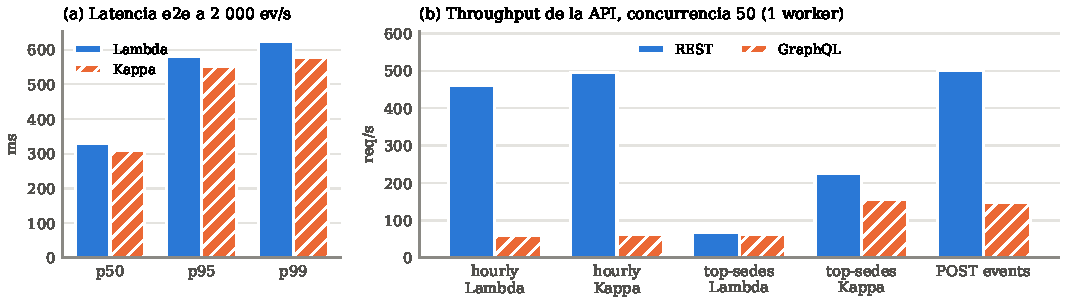
\includegraphics[width=\textwidth]{figs/fig_bench.pdf}
\caption{(a) Latencia de extremo a extremo de la ingesta. (b) Throughput de la API por escenario.}\label{fig:bench}
\end{figure*}

La Tabla~\ref{tab:api} y la Fig.~\ref{fig:bench} muestran la API. Con concurrencia \NumApiCmax, REST
atiende \NumRatioHourly{} veces más peticiones que GraphQL en \emph{hourly}, \NumRatioTop{} veces en
\emph{top-sedes} y \NumRatioPost{} veces en la ingesta. La brecha crece con el tamaño de la respuesta:
el costo está en la validación y serialización campo a campo de GraphQL, no en la base de datos.
Entre vistas, \emph{top-sedes} es \NumTopKappaOverLambda{} veces más rápido sobre Kappa, porque
\texttt{lambda\_serving} debe unir batch y speed en cada consulta.

\section{Discusión}
Persico et~al.~\cite{persico2018} concluyen que Lambda supera a Kappa en análisis de redes sociales en
la nube; aquí Kappa gana en ingesta y en simplicidad (\NumLocKappa{} frente a \NumLocLambda{} líneas
propias y un servicio frente a tres), pero Lambda gana en reproceso, coincidiendo en que el resultado
depende de la carga y del costo de releer el log~\cite{lin2017}. En API, la literatura atribuye a
GraphQL menos esfuerzo de implementación~\cite{brito2020} y respuestas más pequeñas~\cite{brito2019};
este benchmark no contradice eso, pero muestra que en Python esa flexibilidad cuesta rendimiento
cuando el cliente ya pide exactamente lo que el endpoint REST devuelve.

\emph{Amenazas a la validez}: un solo nodo y una VM compartida (Redpanda, PostgreSQL, procesadores y
cliente compiten por CPU); Python como cuello de botella en procesadores y APIs; el volumen real
(\NumEvents{} eventos) es pequeño, por eso la carga constante reemite las mismas marcaciones con
\texttt{produced\_at} actual; las marcaciones de 2020--2021 no reflejan toda la asistencia real,
porque parte se registró por otros medios; y la regla de tardanza es un supuesto.

\section{Conclusión}
Para este caso (volumen moderado, una sola lógica de agregación y necesidad de datos frescos)
conviene \textbf{Kappa}: más throughput, latencia equivalente, menos código y una sola ruta de
cálculo. Lambda se justifica si el reproceso frecuente del histórico es crítico o si la lógica batch
difiere de la de streaming. Para la API conviene \textbf{REST} cuando las consultas son fijas y el
rendimiento importa; GraphQL, cuando hay muchos clientes con necesidades de datos distintas.
Repositorio: \url{https://github.com/mlnp-dev/bi-lambda-kappa-bench}.

\bibliographystyle{IEEEtran}
\bibliography{refs}
\end{document}
